\documentclass[serif,mathserif, 12pt]{beamer}
\usepackage{etex}
\usepackage{amsmath, amsfonts, epsfig, xspace}
\usepackage{algorithm,algorithmic}
\usepackage{pstricks,pst-node}
\usepackage{multimedia}
\usepackage[normal,tight,center]{subfigure}
\setlength{\subfigcapskip}{-.5em}
\usepackage{tkz-euclide}
\usetkzobj{all}
\usepackage{beamerthemesplit}
\usetheme{lankton-keynote}
\usepackage{graphicx,color}
% remove caption of figure
\usepackage[labelformat=empty]{caption}

\usepackage[none]{hyphenat} % hyphenation is ugly in slides
\usepackage{parskip}

\usepackage{relsize} % \smaller to change size

\usepackage{tikz}
\usetikzlibrary{calc}

\usetikzlibrary{arrows}

\newcommand{\TikzDraw}[2][]{
  \begin{tikzpicture}[overlay, remember picture, shift={(current page.center)}, #1]
    #2
  \end{tikzpicture}
}

\newcommand{\gridlines}{
  \TikzDraw{
    \draw[help lines,xstep=.2,ystep=.2,red!20] (current page.south west) grid (current page.north east);
    \draw[help lines,xstep=1,ystep=1,red] (current page.south west) grid (current page.north east);
    \foreach \x in {-15,-14,...,15} {
      \node [anchor=north, red] at (\x,0) {\tiny \x};
      \node [anchor=east,red] at (0,\x) {\tiny \x};
    }
  }
}

\newcommand{\DrawOnImg}[3][]
{
  \begin{tikzpicture}
    \node[anchor=south west,inner sep=0] (image) at (0,0){
      #2
    };
    \begin{scope}[x={(image.south east)},y={(image.north west)}]
      \ifthenelse{\equal{#1}{grid}}
                 {\draw[color=blue, style=dashed] (0,0) grid[xstep=.1, ystep=.1] (1.0001,1.0001);}
                 {}
                 #3
    \end{scope}
  \end{tikzpicture}
}

\usetikzlibrary{matrix}

\newcommand{\BOLD}[1]{\mathbf{#1}}
\newcommand{\BOLDG}[1]{\boldsymbol{#1}}
\newcommand{\PDIF}[2]{\frac{\partial #1}{\partial #2}}
\newcommand{\TODO}[1]{\textcolor{red}{#1}}
\newcommand{\TODOB}[1]{\textcolor{blue}{#1}}
\newcommand{\TODOG}[1]{\textcolor{green!50!black}{#1}}
\newcommand{\argmin}{\operatornamewithlimits{arg\min}}
\DeclareMathOperator{\tr}{tr}
\DeclareMathOperator{\cond}{cond}
\DeclareMathOperator{\ST}{s.t.}
\DeclareMathOperator{\diag}{diag}
\DeclareMathOperator{\Div}{div}
\DeclareMathOperator{\Adv}{Adv}
\DeclareMathOperator{\curl}{curl}

\title[\hspace{2em}\insertframenumber/\inserttotalframenumber]{Scalable Laplacian Eigenfluids}
\date{19th, October 2018}

\author{Theodore Kim et al.}

\makeatletter
\let\@@magyar@captionfix\relax
\makeatother

\begin{document}

\maketitle

\begin{frame}
  \frametitle{Fluid Simulation}
  \begin{itemize}
  \item NS equation
    \[
    \begin{split}
      &\frac{\partial u}{\partial t}+(u\cdot \nabla )u+\frac{1}{\rho}\nabla p
      = f+\nu \Delta u \\
      &\nabla \cdot u = 0
    \end{split}
    \]
   \pause
  \item Discretization method
    \begin{itemize}
    \item[-] Eulerian
    \item[-] Lagrangian
    \item[-] Mixed
    \end{itemize}
  \end{itemize}
\end{frame}

\begin{frame}
  \frametitle{Eulerian method}
  \begin{itemize}
  \item Eulerian method   
    \begin{itemize}
    \item Simple and direct
      \pause
    \item Spatial complexity $O(N^3)$
      \pause
    \item Reduction method?
    \end{itemize}
  \end{itemize}
\end{frame}

\begin{frame}
  \frametitle{Laplacian Eigenfluid [De Witt 2012]}
  \begin{itemize}
  \item Subspace approach
    \[
    u = \sum_{i=1}^r w_i \Psi_i
    \]
  \item<2-> Eigenproblem
    \[
    \begin{split}
      &\Delta \Psi_i = \lambda_i \Psi_i \\
      &\nabla \cdot \Psi_i = 0 \\
      &\Psi_i \cdot n = 0, \text{on~} \partial D
    \end{split}
    \]
  \end{itemize}
  \TikzDraw {
    \visible<3> {
      \node at (0, 0) {
        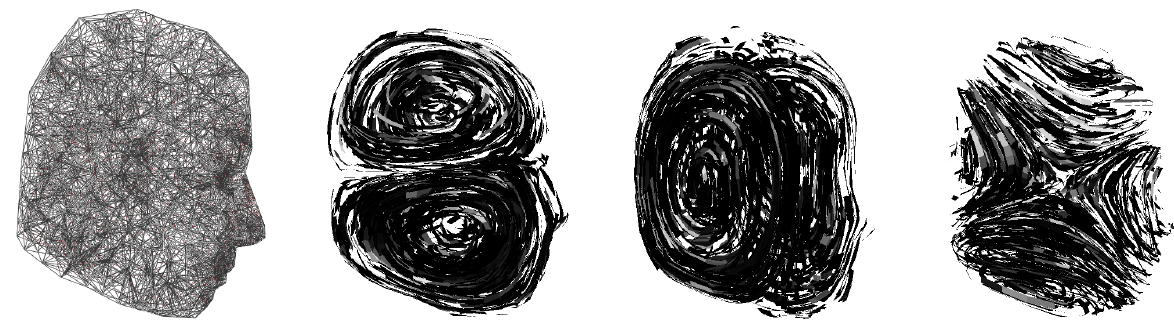
\includegraphics[width=\textwidth]{img/tet_lap_eigen}
      };
    }
  }
\end{frame}

\begin{frame}
  \frametitle{Laplacian Eigenfluid}
  \begin{itemize}
  \item On the square domain $[0, \pi]\times [0, \pi]$
    \[
    \begin{split}
    &\Psi_x(k) = -\frac{1}{\sqrt{k_x^2+k_y^2}}k_y\sin(k_x x) \cos(k_y y) \\
      &\Psi_y(k) = \frac{1}{\sqrt{k_x^2+k_y^2}}k_x\cos(k_x x) \sin(k_y y) \\
      &k_x, k_y \in \mathbb{Z}^+
    \end{split} 
    \]
  \end{itemize}
  \TikzDraw {
    \node at (0, -3) {
      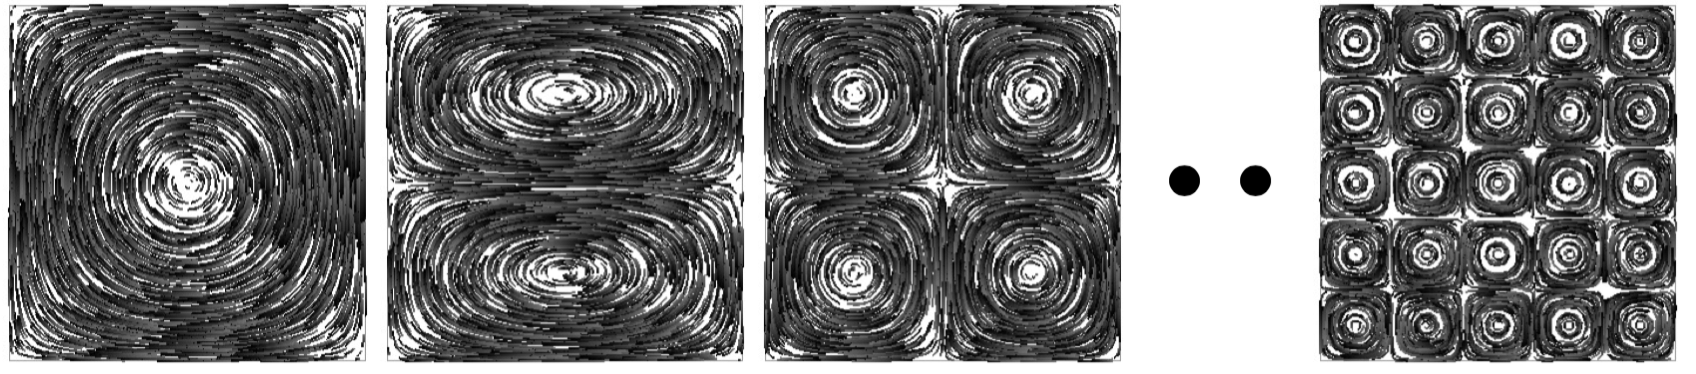
\includegraphics[width=\textwidth]{img/eigenmodes}
    };
  }
\end{frame}

\begin{frame}
  \frametitle{Remarks}
  \begin{itemize}
  \item Vorticity bases
    \[
    \begin{split}
    &\phi_i = \nabla \times \Psi_i \\
    &\omega  = \curl u = \sum_{i=1}^r w_i \phi_i
    \end{split}
    \]
  \item Orthogonality
    \[
    \int_D \|u\|^2 = \sum_i w_i^2
    \]
  \end{itemize}
\end{frame}

\begin{frame}
  \frametitle{Dynamics}
  \begin{itemize}
  \item Vorticity formulation of NS equation
    \[
    \begin{split}
      \dot \omega = \Adv(u, \omega) +\nu \Delta \omega + \curl(f) \\
    \end{split}
    \]
    \item Advection
      \[
      \Adv(u, \omega) = \curl(\omega \times u)
      \]
    \item Galerkin projection
      \[
      \begin{split}
        \sum_k \dot w_k \phi_k = \sum_i \sum_j w_i w_j \Adv(\Psi_i, \phi_j) + &\nu \sum_k w_k \Delta \phi_k +\curl(f) \\
        \visible<2> {&\color{red}{\nu \sum_k w_k \lambda_k \phi_k}}
      \end{split}
      \]
  \end{itemize}
\end{frame}

\begin{frame}
  \frametitle{Dynamics}
  \begin{itemize}
  \item Pair with $\phi_k$
    \[
    \dot w_k = \sum_i\sum_j w_i w_j\langle \Adv(\Psi_i, \phi_j),\phi_k\rangle + \nu \lambda_k w_k  + f_k
    \]
  \item<3> Time integration
    \begin{figure}
      \centering
      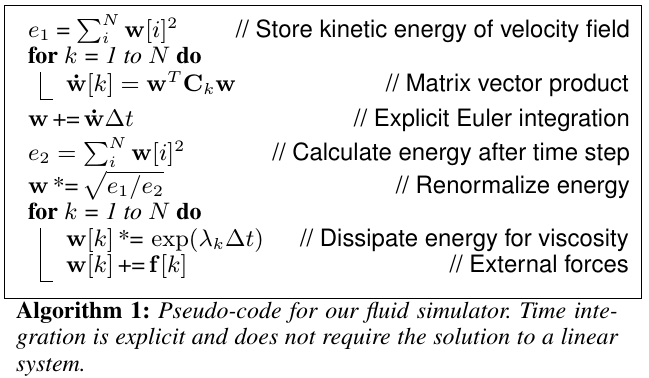
\includegraphics[width=0.6\textwidth]{img/time_integration}
    \end{figure}
  \end{itemize}
  \TikzDraw {
    \visible<2-> {
    \node at (0.5, 1.5) {
      \textcolor{red}{$\mathbb{C}(i, j, k)$}
    };
    }
  }
\end{frame}

\begin{frame}
  \frametitle{Leaving issues}
  \begin{itemize}
  \item Large memory cost $O(rN^3)$
    \pause
  \item Slow evaluation of $Uw$ and $U^Tf$
    \pause
    \begin{itemize}
    \item[-] take up to 84\% of running time
      \pause
    \item[-] Calculate basis on the fly is more slower (5$\times$ to 7$\times$)
      \pause
    \end{itemize}
  \item Only Dirichlet boundary condition is considered
    \pause
  \item Stability of explicit integration
    \pause
  \end{itemize}
\end{frame}

\begin{frame}
  \frametitle{Fast Projection and Reconstruction}
  \begin{itemize}
  \item Do we have to store the bases explicitly?
    \[
    \begin{split}
      &\Psi_x(k) = -\frac{1}{\eta_k}k_y\sin(k_x x)\cos(k_y y) \\
      &\Psi_y(k) = \frac{1}{\eta_k}k_x\cos(k_x x)\sin(k_y y)
    \end{split}
    \]
  \item Not necessary.
    \[
    \begin{split}
    &\langle f_x, \Psi_x(k) \rangle = -\frac{1}{\eta_k}\iint_\Omega f_x \sin(k_x x)\cos(k_y y) dxdy \\
    &\langle f_y, \Psi_y(k) \rangle = \frac{1}{\eta_k}\iint_\Omega f_y \cos(k_x x) \sin(k_y y) dxdy
    \end{split}
    \]
  \end{itemize}
\end{frame}

\begin{frame}
  \frametitle{Fast Projection and Reconstruction}
  \begin{itemize}
  \item DST and DCT
    \[
    \begin{split}
      &\langle f_x, \Psi_x(k) \rangle = -\frac{1}{\eta_k}k_y \color{red}{\hat f_x(k)} \\
      &\langle f_y, \Psi_y(k) \rangle = \frac{1}{\eta_k}k_x \color{red} \hat f_y(k) \\
      &\Rightarrow O(r) \text{~memory}
    \end{split}
    \]
  \item Spectral coordinate
    \[
    \mathcal F_{SC}[\kappa_x \sin(k_x x) \cos(k_y y)] = \kappa_x\delta (k_x, k_y)
    \]
  \end{itemize}
\end{frame}

\begin{frame}
  \frametitle{Reconstruction}
  \begin{itemize}
  \item Reconstruction
    \[
    w_i \rightarrow \hat u_x(k) \rightarrow u_x
    \]
  \item Running time complexity
    \[
    O(rN^3) \rightarrow O(N^3\log N)
    \]
  \item One order faster in practice
  \end{itemize}
\end{frame}

\begin{frame}
  \frametitle{Neumann boundary condition}
  \begin{itemize}
  \item General solution to homogeneous Helmholtz equation $\nabla^2 g(x, y) = \lambda_k g(x, y)$
    \[
    g(x, y) = (a\cos(k_x x)+b\sin(k_x x))(c\cos(k_y y)+d\sin(k_y y))
    \]
  \item Velocity Eigenfunctions
    \[
    \begin{split}
      &\Psi_x(k) =  (a_x\cos(k_x x)+b_x\sin(k_x x))(c_x\cos(k_y y)+d_x\sin(k_y y)) \\
      &\Psi_y(k) =  (a_y\cos(k_x x)+b_y\sin(k_x x))(c_y\cos(k_y y)+d_y\sin(k_y y))
    \end{split}
    \]
  \end{itemize}
\end{frame}

\begin{frame}
  \frametitle{Neumann boundary condition}
  \begin{itemize}
  \item Divergence free $\nabla \cdot \Psi = 0$
    \[
    \begin{split}
      &k_xb_xc_x + k_ya_yd_y = 0,\quad k_xb_xd_x-k_ya_yc_y = 0 \\
      &-k_xa_xc_x + k_yb_yd_y = 0, \quad k_xa_xd_x+k_yb_yc_y = 0
    \end{split}
    \]
  \item Conditions that minimize the number of DST and DCT
    \[
    \begin{split}
      a_xb_x = 0, \quad c_yd_y = 0 \\
      a_yb_y = 0, \quad c_xd_x = 0
    \end{split}
    \]
  \end{itemize}
\end{frame}

\begin{frame}
  \frametitle{Neumann boundary conditions}
  \begin{itemize}
  \item Two Nuemann boundary conditions
    \[
    \frac{\partial \Psi_x}{\partial x}\big|_{x=0,\pi} = 0, \quad\quad \Psi_y\big |_{y=0, \pi} = 0
    \]
  \item Resulted eigenfunctions
    \[
    \boxed{
    \begin{split}
      \Psi_x(k) = \frac{1}{\eta_k}k_y\cos(k_x x)\cos(k_y y) \\
      \Psi_y(k) = \frac{1}{\eta_k}k_x\sin(k_x x)\sin(k_y y)
    \end{split}
    }
    \]
    \visible<2> {
    \begin{figure}
      \centering
      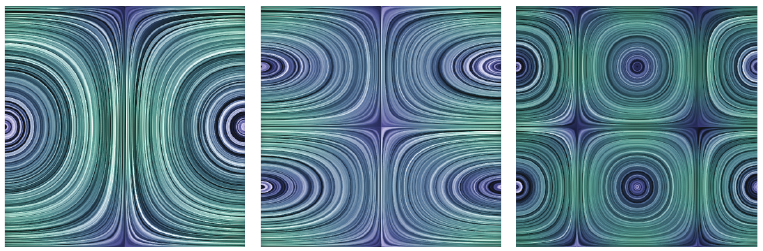
\includegraphics[width=0.7\textwidth]{img/neu_boundary}
    \end{figure}
    }
  \end{itemize}
\end{frame}

\begin{frame}
  \frametitle{Implicit time integration}
  \begin{itemize}
  \item Implicit trapezoidal update
    \[
    \begin{split}
      &w^{t+1} = \frac{h}{2}C^{t+1}w^{t+1} +\frac{h}{2}C^t w^t + w^t+\hat f \\
      &C^{t+1} = \mathbb{C}\times_3 w^{t+1} \\
      &C^{t} = \mathbb{C}\times_3 w^{t}
    \end{split}    
    \]
  \item<2-> Unsymmetric system matrix $I-\frac{h}{2}C^{t+1}$
    \pause
  \item<3-> Normal equation
    \[
    (I-\frac{h}{2}C)^T(I-\frac{h}{2}C) = I+\frac{h^2}{4}C^TC
    \]
  \end{itemize}
  \TikzDraw {
  \visible<4> {
    \node at (0, 0) {
      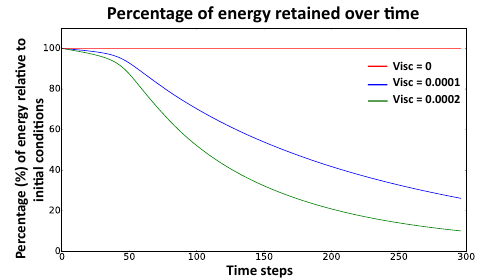
\includegraphics[width=0.7\textwidth]{img/energy_profile}
    };
  }
  }
\end{frame}

\begin{frame} 
  \TikzDraw {
    \node at (0, 0.5) {\Huge{Results}};
  }
  %\gridlines
\end{frame}

\begin{frame}
  \frametitle{Performance}
  \begin{figure}
    \centering
    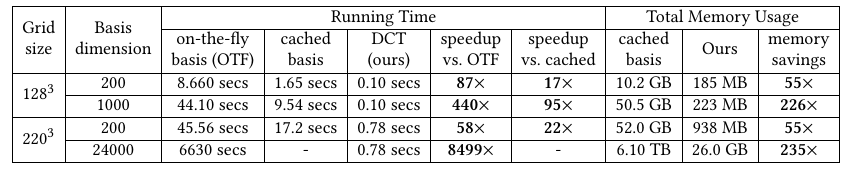
\includegraphics[width=\textwidth]{img/performance}
  \end{figure}
\end{frame}

\begin{frame}
  \begin{figure}
    \centering
    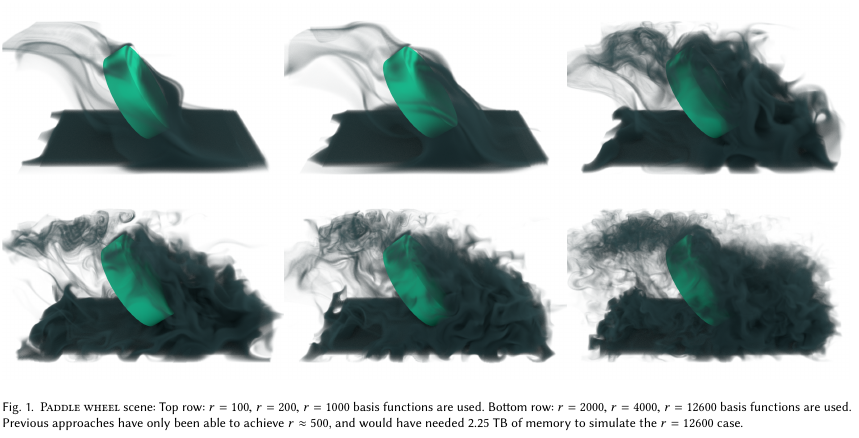
\includegraphics[width=\textwidth]{img/teaser}
  \end{figure}
  \TikzDraw {
    \node at (0, 4) {\color{red}{$r=200$}};
    \node at (-3.5, 4) {\color{red}{$r=100$}};
    \node at (3.5, 4) {\color{red}{$r=1000$}};
    \node at (-3.5, 1.2) {\color{red}{$r=2000$}};
    \node at (0, 1.2) {\color{red}{$r=4000$}};
    \node at (3.5, 1.2) {\color{red}{$r=12600$}};
  }
\end{frame}

\begin{frame}
  \frametitle{Thin Dirichlet obstacles}
  \begin{figure}
    \centering
    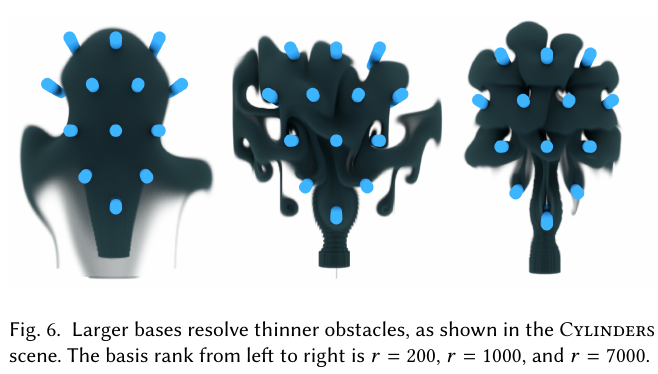
\includegraphics[width=\textwidth]{img/smoke_obs}
  \end{figure}
\end{frame}

\begin{frame}
  \frametitle{Interactive example}
  \TikzDraw {
    \node at (0, 0) {
      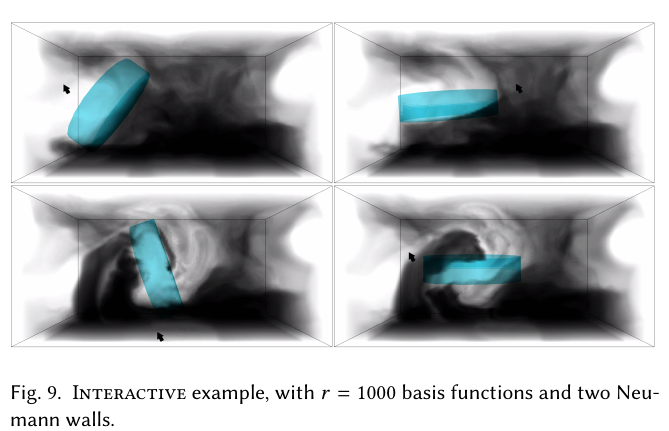
\includegraphics[width=\textwidth]{img/interactive_example}
    };
    \node at (0, -3.5) {
      \textcolor{red}{0.076 secs/frame}
    };
  }
\end{frame}

\begin{frame}
  \frametitle{Future works}
  \begin{itemize}
  \item Extension to include liquid surface
  \item Irregular domain
  \end{itemize}
\end{frame}

\begin{frame} 
  \TikzDraw {
    \node at (0, 0.5) {\Huge{Thanks!}};
  }
  %\gridlines
\end{frame}

\end{document}
